\documentclass[1p]{elsarticle_modified}
%\bibliographystyle{elsarticle-num}

%\usepackage[colorlinks]{hyperref}
%\usepackage{abbrmath_seonhwa} %\Abb, \Ascr, \Acal ,\Abf, \Afrak
\usepackage{amsfonts}
\usepackage{amssymb}
\usepackage{amsmath}
\usepackage{amsthm}
\usepackage{scalefnt}
\usepackage{amsbsy}
\usepackage{kotex}
\usepackage{caption}
\usepackage{subfig}
\usepackage{color}
\usepackage{graphicx}
\usepackage{xcolor} %% white, black, red, green, blue, cyan, magenta, yellow
\usepackage{float}
\usepackage{setspace}
\usepackage{hyperref}

\usepackage{tikz}
\usetikzlibrary{arrows}

\usepackage{multirow}
\usepackage{array} % fixed length table
\usepackage{hhline}

%%%%%%%%%%%%%%%%%%%%%
\makeatletter
\renewcommand*\env@matrix[1][\arraystretch]{%
	\edef\arraystretch{#1}%
	\hskip -\arraycolsep
	\let\@ifnextchar\new@ifnextchar
	\array{*\c@MaxMatrixCols c}}
\makeatother %https://tex.stackexchange.com/questions/14071/how-can-i-increase-the-line-spacing-in-a-matrix
%%%%%%%%%%%%%%%

\usepackage[normalem]{ulem}

\newcommand{\msout}[1]{\ifmmode\text{\sout{\ensuremath{#1}}}\else\sout{#1}\fi}
%SOURCE: \msout is \stkout macro in https://tex.stackexchange.com/questions/20609/strikeout-in-math-mode

\newcommand{\cancel}[1]{
	\ifmmode
	{\color{red}\msout{#1}}
	\else
	{\color{red}\sout{#1}}
	\fi
}

\newcommand{\add}[1]{
	{\color{blue}\uwave{#1}}
}

\newcommand{\replace}[2]{
	\ifmmode
	{\color{red}\msout{#1}}{\color{blue}\uwave{#2}}
	\else
	{\color{red}\sout{#1}}{\color{blue}\uwave{#2}}
	\fi
}

\newcommand{\Sol}{\mathcal{S}} %segment
\newcommand{\D}{D} %diagram
\newcommand{\A}{\mathcal{A}} %arc


%%%%%%%%%%%%%%%%%%%%%%%%%%%%%5 test

\def\sl{\operatorname{\textup{SL}}(2,\Cbb)}
\def\psl{\operatorname{\textup{PSL}}(2,\Cbb)}
\def\quan{\mkern 1mu \triangleright \mkern 1mu}

\theoremstyle{definition}
\newtheorem{thm}{Theorem}[section]
\newtheorem{prop}[thm]{Proposition}
\newtheorem{lem}[thm]{Lemma}
\newtheorem{ques}[thm]{Question}
\newtheorem{cor}[thm]{Corollary}
\newtheorem{defn}[thm]{Definition}
\newtheorem{exam}[thm]{Example}
\newtheorem{rmk}[thm]{Remark}
\newtheorem{alg}[thm]{Algorithm}

\newcommand{\I}{\sqrt{-1}}
\begin{document}

%\begin{frontmatter}
%
%\title{Boundary parabolic representations of knots up to 8 crossings}
%
%%% Group authors per affiliation:
%\author{Yunhi Cho} 
%\address{Department of Mathematics, University of Seoul, Seoul, Korea}
%\ead{yhcho@uos.ac.kr}
%
%
%\author{Seonhwa Kim} %\fnref{s_kim}}
%\address{Center for Geometry and Physics, Institute for Basic Science, Pohang, 37673, Korea}
%\ead{ryeona17@ibs.re.kr}
%
%\author{Hyuk Kim}
%\address{Department of Mathematical Sciences, Seoul National University, Seoul 08826, Korea}
%\ead{hyukkim@snu.ac.kr}
%
%\author{Seokbeom Yoon}
%\address{Department of Mathematical Sciences, Seoul National University, Seoul, 08826,  Korea}
%\ead{sbyoon15@snu.ac.kr}
%
%\begin{abstract}
%We find all boundary parabolic representation of knots up to 8 crossings.
%
%\end{abstract}
%\begin{keyword}
%    \MSC[2010] 57M25 
%\end{keyword}
%
%\end{frontmatter}

%\linenumbers
%\tableofcontents
%
\newcommand\colored[1]{\textcolor{white}{\rule[-0.35ex]{0.8em}{1.4ex}}\kern-0.8em\color{red} #1}%
%\newcommand\colored[1]{\textcolor{white}{ #1}\kern-2.17ex	\textcolor{white}{ #1}\kern-1.81ex	\textcolor{white}{ #1}\kern-2.15ex\color{red}#1	}

{\Large $\underline{12n_{0450}~(K12n_{0450})}$}

\setlength{\tabcolsep}{10pt}
\renewcommand{\arraystretch}{1.6}
\vspace{1cm}\begin{tabular}{m{100pt}>{\centering\arraybackslash}m{274pt}}
\multirow{5}{120pt}{
	\centering
	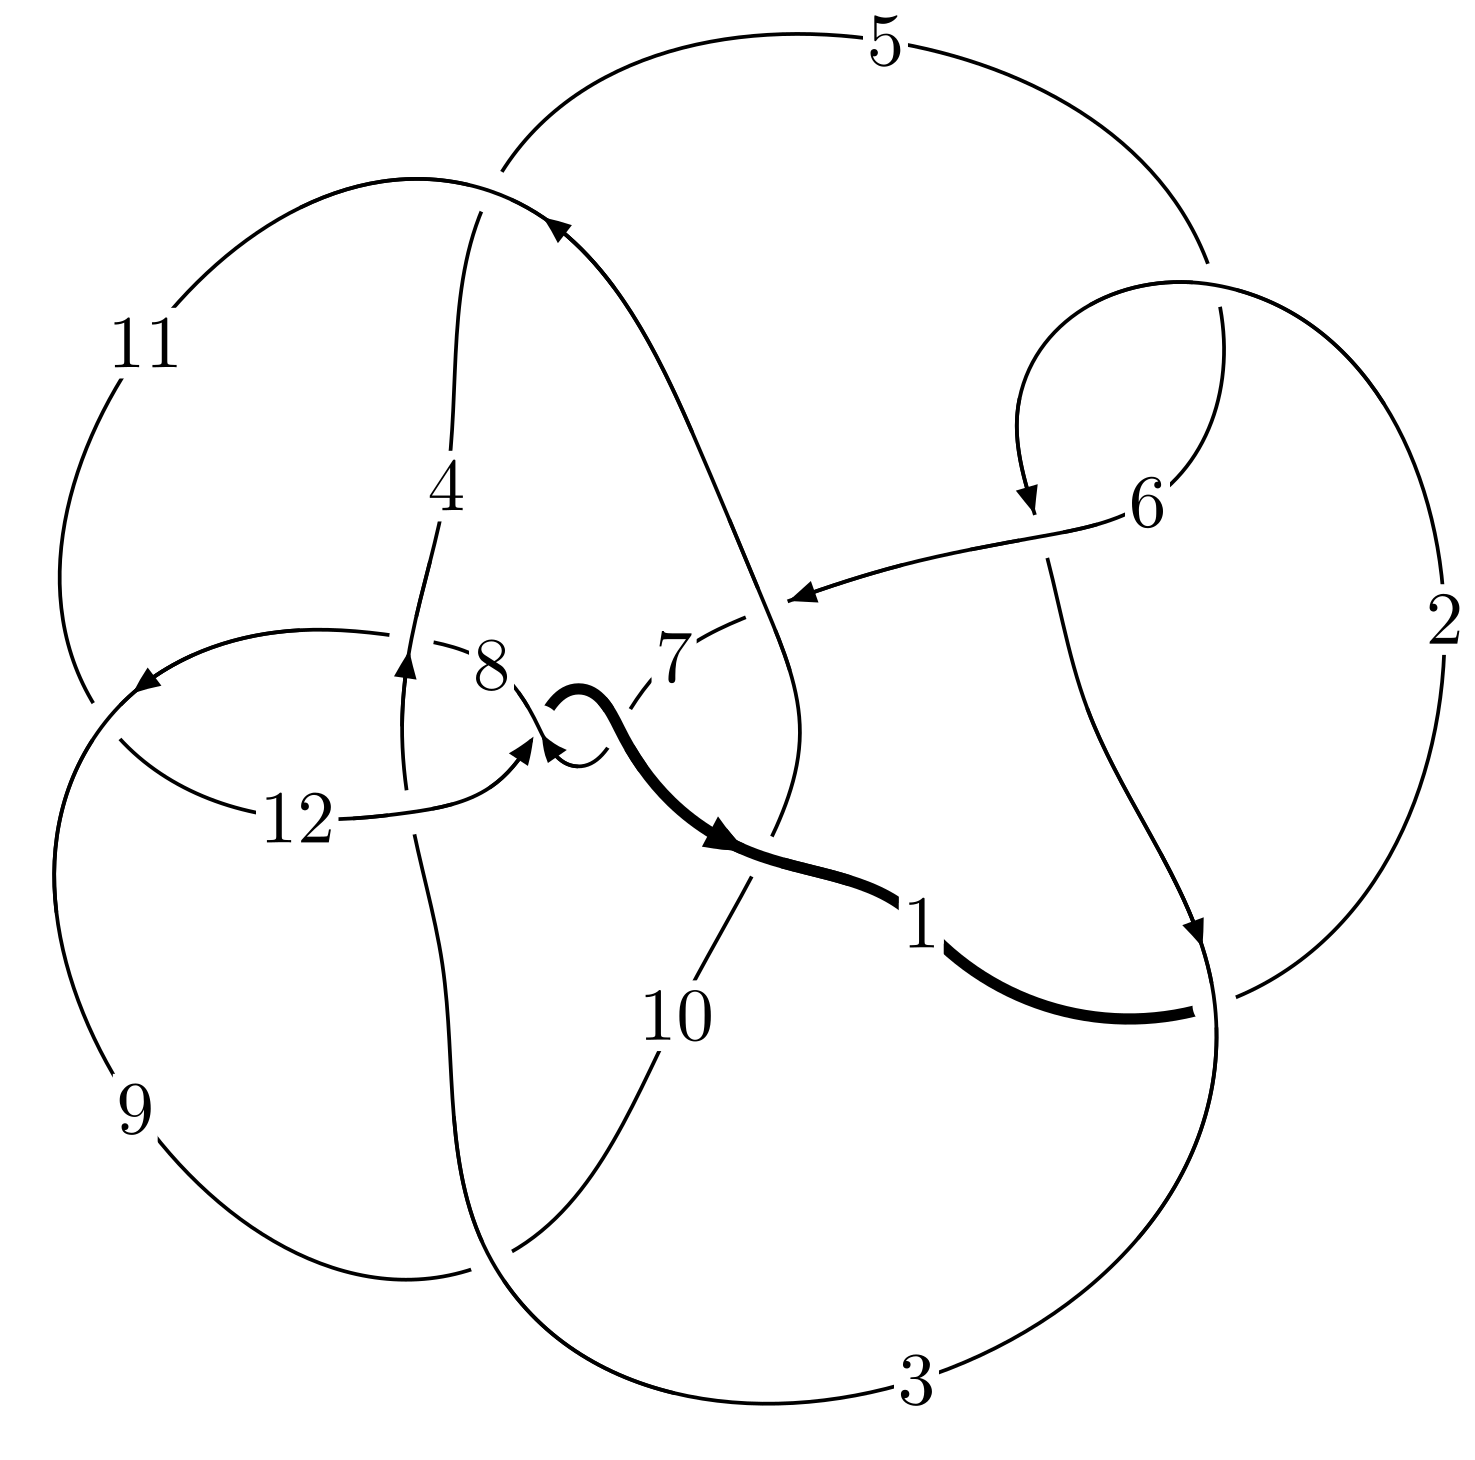
\includegraphics[width=112pt]{../../../GIT/diagram.site/Diagrams/png/2539_12n_0450.png}\\
\ \ \ A knot diagram\footnotemark}&
\allowdisplaybreaks
\textbf{Linearized knot diagam} \\
\cline{2-2}
 &
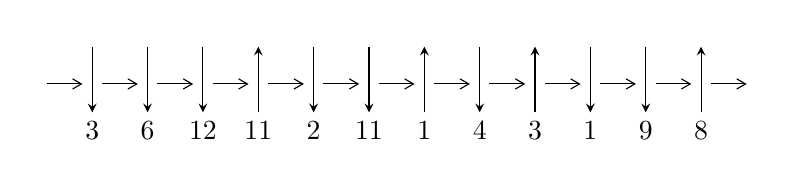
\begin{tikzpicture}[x=20pt, y=17pt]
	% nodes
	\node (C0) at (0, 0) {};
	\node (C1) at (1, 0) {};
	\node (C1U) at (1, +1) {};
	\node (C1D) at (1, -1) {3};

	\node (C2) at (2, 0) {};
	\node (C2U) at (2, +1) {};
	\node (C2D) at (2, -1) {6};

	\node (C3) at (3, 0) {};
	\node (C3U) at (3, +1) {};
	\node (C3D) at (3, -1) {12};

	\node (C4) at (4, 0) {};
	\node (C4U) at (4, +1) {};
	\node (C4D) at (4, -1) {11};

	\node (C5) at (5, 0) {};
	\node (C5U) at (5, +1) {};
	\node (C5D) at (5, -1) {2};

	\node (C6) at (6, 0) {};
	\node (C6U) at (6, +1) {};
	\node (C6D) at (6, -1) {11};

	\node (C7) at (7, 0) {};
	\node (C7U) at (7, +1) {};
	\node (C7D) at (7, -1) {1};

	\node (C8) at (8, 0) {};
	\node (C8U) at (8, +1) {};
	\node (C8D) at (8, -1) {4};

	\node (C9) at (9, 0) {};
	\node (C9U) at (9, +1) {};
	\node (C9D) at (9, -1) {3};

	\node (C10) at (10, 0) {};
	\node (C10U) at (10, +1) {};
	\node (C10D) at (10, -1) {1};

	\node (C11) at (11, 0) {};
	\node (C11U) at (11, +1) {};
	\node (C11D) at (11, -1) {9};

	\node (C12) at (12, 0) {};
	\node (C12U) at (12, +1) {};
	\node (C12D) at (12, -1) {8};
	\node (C13) at (13, 0) {};

	% arrows
	\draw[->,>={angle 60}]
	(C0) edge (C1) (C1) edge (C2) (C2) edge (C3) (C3) edge (C4) (C4) edge (C5) (C5) edge (C6) (C6) edge (C7) (C7) edge (C8) (C8) edge (C9) (C9) edge (C10) (C10) edge (C11) (C11) edge (C12) (C12) edge (C13) ;	\draw[->,>=stealth]
	(C1U) edge (C1D) (C2U) edge (C2D) (C3U) edge (C3D) (C4D) edge (C4U) (C5U) edge (C5D) (C6U) edge (C6D) (C7D) edge (C7U) (C8U) edge (C8D) (C9D) edge (C9U) (C10U) edge (C10D) (C11U) edge (C11D) (C12D) edge (C12U) ;
	\end{tikzpicture} \\
\hhline{~~} \\& 
\textbf{Solving Sequence} \\ \cline{2-2} 
 &
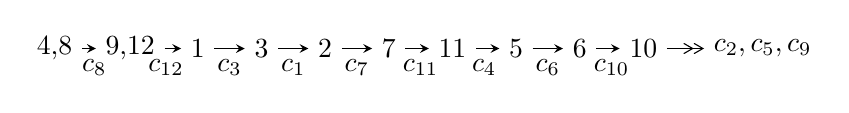
\begin{tikzpicture}[x=23pt, y=7pt]
	% node
	\node (A0) at (-1/8, 0) {4,8};
	\node (A1) at (17/16, 0) {9,12};
	\node (A2) at (17/8, 0) {1};
	\node (A3) at (25/8, 0) {3};
	\node (A4) at (33/8, 0) {2};
	\node (A5) at (41/8, 0) {7};
	\node (A6) at (49/8, 0) {11};
	\node (A7) at (57/8, 0) {5};
	\node (A8) at (65/8, 0) {6};
	\node (A9) at (73/8, 0) {10};
	\node (C1) at (1/2, -1) {$c_{8}$};
	\node (C2) at (13/8, -1) {$c_{12}$};
	\node (C3) at (21/8, -1) {$c_{3}$};
	\node (C4) at (29/8, -1) {$c_{1}$};
	\node (C5) at (37/8, -1) {$c_{7}$};
	\node (C6) at (45/8, -1) {$c_{11}$};
	\node (C7) at (53/8, -1) {$c_{4}$};
	\node (C8) at (61/8, -1) {$c_{6}$};
	\node (C9) at (69/8, -1) {$c_{10}$};
	\node (A10) at (11, 0) {$c_{2},c_{5},c_{9}$};

	% edge
	\draw[->,>=stealth]	
	(A0) edge (A1) (A1) edge (A2) (A2) edge (A3) (A3) edge (A4) (A4) edge (A5) (A5) edge (A6) (A6) edge (A7) (A7) edge (A8) (A8) edge (A9) ;
	\draw[->>,>={angle 60}]	
	(A9) edge (A10);
\end{tikzpicture} \\ 

\end{tabular} \\

\footnotetext{
The image of knot diagram is generated by the software ``\textbf{Draw programme}" developed by Andrew Bartholomew(\url{http://www.layer8.co.uk/maths/draw/index.htm\#Running-draw}), where we modified some parts for our purpose(\url{https://github.com/CATsTAILs/LinksPainter}).
}\phantom \\ \newline 
\centering \textbf{Ideals for irreducible components\footnotemark of $X_{\text{par}}$} 
 
\begin{align*}
I^u_{1}&=\langle 
-1.60444\times10^{22} u^{28}+2.55663\times10^{22} u^{27}+\cdots+2.54971\times10^{22} b-4.79237\times10^{21},\;a-1,\\
\phantom{I^u_{1}}&\phantom{= \langle  }u^{29}-2 u^{28}+\cdots-3 u+1\rangle \\
I^u_{2}&=\langle 
-101 u^{19}+163 u^{18}+\cdots+83 b-171,\;a+1,\;u^{20}+u^{19}+\cdots-2 u+1\rangle \\
I^u_{3}&=\langle 
-3.73965\times10^{51} u^{39}-8.54778\times10^{51} u^{38}+\cdots+4.04316\times10^{50} b+1.36063\times10^{52},\\
\phantom{I^u_{3}}&\phantom{= \langle  }-3.50215\times10^{83} u^{39}-8.75016\times10^{83} u^{38}+\cdots+9.39462\times10^{81} a+3.79380\times10^{83},\\
\phantom{I^u_{3}}&\phantom{= \langle  }u^{40}+2 u^{39}+\cdots-13 u+1\rangle \\
I^u_{4}&=\langle 
- u^3-2 u^2+2 b-2 u+1,\;u^3+2 a-5,\;u^4+u^3+2 u^2- u+1\rangle \\
I^u_{5}&=\langle 
b+u+1,\;a-1,\;u^2+u+1\rangle \\
\\
\end{align*}
\raggedright * 5 irreducible components of $\dim_{\mathbb{C}}=0$, with total 95 representations.\\
\footnotetext{All coefficients of polynomials are rational numbers. But the coefficients are sometimes approximated in decimal forms when there is not enough margin.}
\newpage
\renewcommand{\arraystretch}{1}
\centering \section*{I. $I^u_{1}= \langle -1.60\times10^{22} u^{28}+2.56\times10^{22} u^{27}+\cdots+2.55\times10^{22} b-4.79\times10^{21},\;a-1,\;u^{29}-2 u^{28}+\cdots-3 u+1 \rangle$}
\flushleft \textbf{(i) Arc colorings}\\
\begin{tabular}{m{7pt} m{180pt} m{7pt} m{180pt} }
\flushright $a_{4}=$&$\begin{pmatrix}0\\u\end{pmatrix}$ \\
\flushright $a_{8}=$&$\begin{pmatrix}1\\0\end{pmatrix}$ \\
\flushright $a_{9}=$&$\begin{pmatrix}1\\u^2\end{pmatrix}$ \\
\flushright $a_{12}=$&$\begin{pmatrix}1\\0.629264 u^{28}-1.00271 u^{27}+\cdots+4.09043 u+0.187957\end{pmatrix}$ \\
\flushright $a_{1}=$&$\begin{pmatrix}0.629264 u^{28}-1.00271 u^{27}+\cdots+4.09043 u+1.18796\\0.629264 u^{28}-1.00271 u^{27}+\cdots+4.09043 u+0.187957\end{pmatrix}$ \\
\flushright $a_{3}=$&$\begin{pmatrix}u\\0.255815 u^{28}-0.468311 u^{27}+\cdots+3.07575 u-0.629264\end{pmatrix}$ \\
\flushright $a_{2}=$&$\begin{pmatrix}0.572071 u^{28}-0.965425 u^{27}+\cdots+3.54331 u+0.766462\\0.0578442 u^{28}-0.0712994 u^{27}+\cdots+0.481981 u+0.447834\end{pmatrix}$ \\
\flushright $a_{7}=$&$\begin{pmatrix}1.81161 u^{28}-3.20172 u^{27}+\cdots+12.3104 u-1.73946\\1.18234 u^{28}-2.19901 u^{27}+\cdots+8.21997 u-2.92741\end{pmatrix}$ \\
\flushright $a_{11}=$&$\begin{pmatrix}0.629264 u^{28}-1.00271 u^{27}+\cdots+4.09043 u+1.18796\\0.672582 u^{28}-1.03859 u^{27}+\cdots+4.22861 u-0.0678573\end{pmatrix}$ \\
\flushright $a_{5}=$&$\begin{pmatrix}0.575794 u^{28}-1.20888 u^{27}+\cdots+6.02284 u-2.35424\\0.299202 u^{28}-0.691078 u^{27}+\cdots+3.19943 u-1.66768\end{pmatrix}$ \\
\flushright $a_{6}=$&$\begin{pmatrix}1.13473 u^{28}-2.13653 u^{27}+\cdots+8.11688 u-1.69516\\0.493538 u^{28}-1.13834 u^{27}+\cdots+4.35556 u-1.96801\end{pmatrix}$ \\
\flushright $a_{10}=$&$\begin{pmatrix}-0.0433177 u^{28}+0.0358776 u^{27}+\cdots-0.138180 u+1.25581\\0.0355816 u^{28}-0.0476050 u^{27}+\cdots+0.517900 u+0.626552\end{pmatrix}$\\&\end{tabular}
\flushleft \textbf{(ii) Obstruction class $= -1$}\\~\\
\flushleft \textbf{(iii) Cusp Shapes $= -\frac{1968133132746250507567}{25497116697596300834899} u^{28}+\frac{51952197439902261991497}{25497116697596300834899} u^{27}+\cdots-\frac{276922517104029225550000}{25497116697596300834899} u+\frac{47895990870458513606664}{25497116697596300834899}$}\\~\\
\newpage\renewcommand{\arraystretch}{1}
\flushleft \textbf{(iv) u-Polynomials at the component}\newline \\
\begin{tabular}{m{50pt}|m{274pt}}
Crossings & \hspace{64pt}u-Polynomials at each crossing \\
\hline $$\begin{aligned}c_{1}\end{aligned}$$&$\begin{aligned}
&u^{29}+9 u^{28}+\cdots-861 u+441
\end{aligned}$\\
\hline $$\begin{aligned}c_{2},c_{5}\end{aligned}$$&$\begin{aligned}
&u^{29}+9 u^{28}+\cdots+105 u+21
\end{aligned}$\\
\hline $$\begin{aligned}c_{3},c_{8}\end{aligned}$$&$\begin{aligned}
&u^{29}-2 u^{28}+\cdots-3 u+1
\end{aligned}$\\
\hline $$\begin{aligned}c_{4},c_{9}\end{aligned}$$&$\begin{aligned}
&u^{29}- u^{28}+\cdots+19 u+17
\end{aligned}$\\
\hline $$\begin{aligned}c_{6},c_{10}\end{aligned}$$&$\begin{aligned}
&u^{29}+3 u^{28}+\cdots+29 u+1
\end{aligned}$\\
\hline $$\begin{aligned}c_{7},c_{12}\end{aligned}$$&$\begin{aligned}
&u^{29}-18 u^{28}+\cdots-2560 u+512
\end{aligned}$\\
\hline $$\begin{aligned}c_{11}\end{aligned}$$&$\begin{aligned}
&u^{29}-18 u^{28}+\cdots+294 u-21
\end{aligned}$\\
\hline
\end{tabular}\\~\\
\newpage\renewcommand{\arraystretch}{1}
\flushleft \textbf{(v) Riley Polynomials at the component}\newline \\
\begin{tabular}{m{50pt}|m{274pt}}
Crossings & \hspace{64pt}Riley Polynomials at each crossing \\
\hline $$\begin{aligned}c_{1}\end{aligned}$$&$\begin{aligned}
&y^{29}+31 y^{28}+\cdots+2190447 y-194481
\end{aligned}$\\
\hline $$\begin{aligned}c_{2},c_{5}\end{aligned}$$&$\begin{aligned}
&y^{29}-9 y^{28}+\cdots-861 y-441
\end{aligned}$\\
\hline $$\begin{aligned}c_{3},c_{8}\end{aligned}$$&$\begin{aligned}
&y^{29}+28 y^{27}+\cdots-11 y-1
\end{aligned}$\\
\hline $$\begin{aligned}c_{4},c_{9}\end{aligned}$$&$\begin{aligned}
&y^{29}-15 y^{28}+\cdots+3183 y-289
\end{aligned}$\\
\hline $$\begin{aligned}c_{6},c_{10}\end{aligned}$$&$\begin{aligned}
&y^{29}+45 y^{28}+\cdots+331 y-1
\end{aligned}$\\
\hline $$\begin{aligned}c_{7},c_{12}\end{aligned}$$&$\begin{aligned}
&y^{29}+12 y^{28}+\cdots+7864320 y-262144
\end{aligned}$\\
\hline $$\begin{aligned}c_{11}\end{aligned}$$&$\begin{aligned}
&y^{29}+4 y^{28}+\cdots+1344 y-441
\end{aligned}$\\
\hline
\end{tabular}\\~\\
\newpage\flushleft \textbf{(vi) Complex Volumes and Cusp Shapes}
$$\begin{array}{c|c|c}  
\text{Solutions to }I^u_{1}& \I (\text{vol} + \sqrt{-1}CS) & \text{Cusp shape}\\
 \hline 
\begin{aligned}
u &= -0.553569 + 0.834452 I \\
a &= \phantom{-}1.00000\phantom{ +0.000000I} \\
b &= -1.086080 - 0.257296 I\end{aligned}
 & \phantom{-}1.07593 + 3.51673 I & -0.88547 - 6.06083 I \\ \hline\begin{aligned}
u &= -0.553569 - 0.834452 I \\
a &= \phantom{-}1.00000\phantom{ +0.000000I} \\
b &= -1.086080 + 0.257296 I\end{aligned}
 & \phantom{-}1.07593 - 3.51673 I & -0.88547 + 6.06083 I \\ \hline\begin{aligned}
u &= -0.898744 + 0.481411 I \\
a &= \phantom{-}1.00000\phantom{ +0.000000I} \\
b &= -1.04286 - 1.29908 I\end{aligned}
 & \phantom{-}4.54760 + 1.43626 I & -5.55282 - 2.76214 I \\ \hline\begin{aligned}
u &= -0.898744 - 0.481411 I \\
a &= \phantom{-}1.00000\phantom{ +0.000000I} \\
b &= -1.04286 + 1.29908 I\end{aligned}
 & \phantom{-}4.54760 - 1.43626 I & -5.55282 + 2.76214 I \\ \hline\begin{aligned}
u &= \phantom{-}0.885586 + 0.378627 I \\
a &= \phantom{-}1.00000\phantom{ +0.000000I} \\
b &= -1.05204 + 1.35554 I\end{aligned}
 & \phantom{-}4.49815 - 7.86181 I & -6.63470 + 7.85058 I \\ \hline\begin{aligned}
u &= \phantom{-}0.885586 - 0.378627 I \\
a &= \phantom{-}1.00000\phantom{ +0.000000I} \\
b &= -1.05204 - 1.35554 I\end{aligned}
 & \phantom{-}4.49815 + 7.86181 I & -6.63470 - 7.85058 I \\ \hline\begin{aligned}
u &= \phantom{-}0.390658 + 0.859931 I \\
a &= \phantom{-}1.00000\phantom{ +0.000000I} \\
b &= -0.766543 - 0.146226 I\end{aligned}
 & \phantom{-}2.79783 + 0.59845 I & \phantom{-}2.09571 - 1.89566 I \\ \hline\begin{aligned}
u &= \phantom{-}0.390658 - 0.859931 I \\
a &= \phantom{-}1.00000\phantom{ +0.000000I} \\
b &= -0.766543 + 0.146226 I\end{aligned}
 & \phantom{-}2.79783 - 0.59845 I & \phantom{-}2.09571 + 1.89566 I \\ \hline\begin{aligned}
u &= -0.631994 + 0.882834 I \\
a &= \phantom{-}1.00000\phantom{ +0.000000I} \\
b &= -1.47686 + 0.36781 I\end{aligned}
 & \phantom{-}9.81309 + 8.93318 I & -1.43468 - 7.09429 I \\ \hline\begin{aligned}
u &= -0.631994 - 0.882834 I \\
a &= \phantom{-}1.00000\phantom{ +0.000000I} \\
b &= -1.47686 - 0.36781 I\end{aligned}
 & \phantom{-}9.81309 - 8.93318 I & -1.43468 + 7.09429 I\\
 \hline 
 \end{array}$$\newpage$$\begin{array}{c|c|c}  
\text{Solutions to }I^u_{1}& \I (\text{vol} + \sqrt{-1}CS) & \text{Cusp shape}\\
 \hline 
\begin{aligned}
u &= \phantom{-}0.622317 + 0.918963 I \\
a &= \phantom{-}1.00000\phantom{ +0.000000I} \\
b &= -1.37238 - 0.35412 I\end{aligned}
 & \phantom{-}10.54740 - 2.08899 I & -0.28693 + 2.13318 I \\ \hline\begin{aligned}
u &= \phantom{-}0.622317 - 0.918963 I \\
a &= \phantom{-}1.00000\phantom{ +0.000000I} \\
b &= -1.37238 + 0.35412 I\end{aligned}
 & \phantom{-}10.54740 + 2.08899 I & -0.28693 - 2.13318 I \\ \hline\begin{aligned}
u &= -0.246064 + 0.681299 I \\
a &= \phantom{-}1.00000\phantom{ +0.000000I} \\
b &= -0.291258 - 0.850239 I\end{aligned}
 & -0.06368 + 1.78512 I & -1.17437 - 4.76019 I \\ \hline\begin{aligned}
u &= -0.246064 - 0.681299 I \\
a &= \phantom{-}1.00000\phantom{ +0.000000I} \\
b &= -0.291258 + 0.850239 I\end{aligned}
 & -0.06368 - 1.78512 I & -1.17437 + 4.76019 I \\ \hline\begin{aligned}
u &= \phantom{-}1.040160 + 0.774644 I \\
a &= \phantom{-}1.00000\phantom{ +0.000000I} \\
b &= \phantom{-}0.003744 + 1.185610 I\end{aligned}
 & -4.83952 + 0.52966 I & -8.94722 - 4.42653 I \\ \hline\begin{aligned}
u &= \phantom{-}1.040160 - 0.774644 I \\
a &= \phantom{-}1.00000\phantom{ +0.000000I} \\
b &= \phantom{-}0.003744 - 1.185610 I\end{aligned}
 & -4.83952 - 0.52966 I & -8.94722 + 4.42653 I \\ \hline\begin{aligned}
u &= -0.662685\phantom{ +0.000000I} \\
a &= \phantom{-}1.00000\phantom{ +0.000000I} \\
b &= \phantom{-}0.179578\phantom{ +0.000000I}\end{aligned}
 & -1.45974\phantom{ +0.000000I} & -5.50510\phantom{ +0.000000I} \\ \hline\begin{aligned}
u &= -0.954244 + 0.980591 I \\
a &= \phantom{-}1.00000\phantom{ +0.000000I} \\
b &= -0.384074 - 1.189700 I\end{aligned}
 & -0.41230 + 3.60972 I & -1.66995 - 2.14870 I \\ \hline\begin{aligned}
u &= -0.954244 - 0.980591 I \\
a &= \phantom{-}1.00000\phantom{ +0.000000I} \\
b &= -0.384074 + 1.189700 I\end{aligned}
 & -0.41230 - 3.60972 I & -1.66995 + 2.14870 I \\ \hline\begin{aligned}
u &= \phantom{-}0.447072 + 0.358702 I \\
a &= \phantom{-}1.00000\phantom{ +0.000000I} \\
b &= -0.44229 + 1.60778 I\end{aligned}
 & -2.94431 - 4.31709 I & -9.8550 + 12.7269 I\\
 \hline 
 \end{array}$$\newpage$$\begin{array}{c|c|c}  
\text{Solutions to }I^u_{1}& \I (\text{vol} + \sqrt{-1}CS) & \text{Cusp shape}\\
 \hline 
\begin{aligned}
u &= \phantom{-}0.447072 - 0.358702 I \\
a &= \phantom{-}1.00000\phantom{ +0.000000I} \\
b &= -0.44229 - 1.60778 I\end{aligned}
 & -2.94431 + 4.31709 I & -9.8550 - 12.7269 I \\ \hline\begin{aligned}
u &= \phantom{-}1.08646 + 1.01922 I \\
a &= \phantom{-}1.00000\phantom{ +0.000000I} \\
b &= -0.47265 + 1.42228 I\end{aligned}
 & -4.10333 - 8.99973 I & -2.77388 + 6.56416 I \\ \hline\begin{aligned}
u &= \phantom{-}1.08646 - 1.01922 I \\
a &= \phantom{-}1.00000\phantom{ +0.000000I} \\
b &= -0.47265 - 1.42228 I\end{aligned}
 & -4.10333 + 8.99973 I & -2.77388 - 6.56416 I \\ \hline\begin{aligned}
u &= -1.16230 + 1.12800 I \\
a &= \phantom{-}1.00000\phantom{ +0.000000I} \\
b &= -0.74251 - 1.33081 I\end{aligned}
 & \phantom{-}7.38506 + 9.34813 I & -2.85483 - 4.48281 I \\ \hline\begin{aligned}
u &= -1.16230 - 1.12800 I \\
a &= \phantom{-}1.00000\phantom{ +0.000000I} \\
b &= -0.74251 + 1.33081 I\end{aligned}
 & \phantom{-}7.38506 - 9.34813 I & -2.85483 + 4.48281 I \\ \hline\begin{aligned}
u &= \phantom{-}0.117027 + 0.360629 I \\
a &= \phantom{-}1.00000\phantom{ +0.000000I} \\
b &= \phantom{-}0.817618 + 0.957619 I\end{aligned}
 & -2.13866 + 1.52424 I & -4.33983 - 3.48956 I \\ \hline\begin{aligned}
u &= \phantom{-}0.117027 - 0.360629 I \\
a &= \phantom{-}1.00000\phantom{ +0.000000I} \\
b &= \phantom{-}0.817618 - 0.957619 I\end{aligned}
 & -2.13866 - 1.52424 I & -4.33983 + 3.48956 I \\ \hline\begin{aligned}
u &= \phantom{-}1.18898 + 1.11285 I \\
a &= \phantom{-}1.00000\phantom{ +0.000000I} \\
b &= -0.78159 + 1.34575 I\end{aligned}
 & \phantom{-}6.6428 - 16.5676 I & -4.00000 + 8.49370 I \\ \hline\begin{aligned}
u &= \phantom{-}1.18898 - 1.11285 I \\
a &= \phantom{-}1.00000\phantom{ +0.000000I} \\
b &= -0.78159 - 1.34575 I\end{aligned}
 & \phantom{-}6.6428 + 16.5676 I & -4.00000 - 8.49370 I\\
 \hline 
 \end{array}$$\newpage\newpage\renewcommand{\arraystretch}{1}
\centering \section*{II. $I^u_{2}= \langle -101 u^{19}+163 u^{18}+\cdots+83 b-171,\;a+1,\;u^{20}+u^{19}+\cdots-2 u+1 \rangle$}
\flushleft \textbf{(i) Arc colorings}\\
\begin{tabular}{m{7pt} m{180pt} m{7pt} m{180pt} }
\flushright $a_{4}=$&$\begin{pmatrix}0\\u\end{pmatrix}$ \\
\flushright $a_{8}=$&$\begin{pmatrix}1\\0\end{pmatrix}$ \\
\flushright $a_{9}=$&$\begin{pmatrix}1\\u^2\end{pmatrix}$ \\
\flushright $a_{12}=$&$\begin{pmatrix}-1\\1.21687 u^{19}-1.96386 u^{18}+\cdots-10.1928 u+2.06024\end{pmatrix}$ \\
\flushright $a_{1}=$&$\begin{pmatrix}1.21687 u^{19}-1.96386 u^{18}+\cdots-10.1928 u+1.06024\\1.21687 u^{19}-1.96386 u^{18}+\cdots-10.1928 u+2.06024\end{pmatrix}$ \\
\flushright $a_{3}=$&$\begin{pmatrix}u\\3.18072 u^{19}+2.53012 u^{18}+\cdots-3.49398 u+1.21687\end{pmatrix}$ \\
\flushright $a_{2}=$&$\begin{pmatrix}2.16867 u^{19}-2.63855 u^{18}+\cdots-15.9277 u+4.60241\\2.15663 u^{19}-3.80723 u^{18}+\cdots-19.3614 u+8.98795\end{pmatrix}$ \\
\flushright $a_{7}=$&$\begin{pmatrix}1.34940 u^{19}+4.89157 u^{18}+\cdots+7.57831 u-11.1807\\2.56627 u^{19}+2.92771 u^{18}+\cdots-2.61446 u-10.1205\end{pmatrix}$ \\
\flushright $a_{11}=$&$\begin{pmatrix}1.21687 u^{19}-1.96386 u^{18}+\cdots-10.1928 u+1.06024\\1.86747 u^{19}-3.85542 u^{18}+\cdots-17.7711 u+5.24096\end{pmatrix}$ \\
\flushright $a_{5}=$&$\begin{pmatrix}1.63855 u^{19}+1.93976 u^{18}+\cdots-4.01205 u-1.43373\\-0.626506 u^{19}+0.228916 u^{18}+\cdots-0.554217 u-2.95181\end{pmatrix}$ \\
\flushright $a_{6}=$&$\begin{pmatrix}-0.168675 u^{19}+5.63855 u^{18}+\cdots+15.9277 u-10.6024\\-0.156627 u^{19}+6.80723 u^{18}+\cdots+19.3614 u-15.9880\end{pmatrix}$ \\
\flushright $a_{10}=$&$\begin{pmatrix}0.650602 u^{19}-1.89157 u^{18}+\cdots-7.57831 u+4.18072\\0.650602 u^{19}-1.89157 u^{18}+\cdots-7.57831 u+4.18072\end{pmatrix}$\\&\end{tabular}
\flushleft \textbf{(ii) Obstruction class $= 1$}\\~\\
\flushleft \textbf{(iii) Cusp Shapes $= -\frac{1728}{83} u^{19}-\frac{2529}{83} u^{18}+\cdots-\frac{290}{83} u-\frac{148}{83}$}\\~\\
\newpage\renewcommand{\arraystretch}{1}
\flushleft \textbf{(iv) u-Polynomials at the component}\newline \\
\begin{tabular}{m{50pt}|m{274pt}}
Crossings & \hspace{64pt}u-Polynomials at each crossing \\
\hline $$\begin{aligned}c_{1}\end{aligned}$$&$\begin{aligned}
&u^{20}-8 u^{19}+\cdots-10 u+1
\end{aligned}$\\
\hline $$\begin{aligned}c_{2}\end{aligned}$$&$\begin{aligned}
&u^{20}+4 u^{19}+\cdots+4 u+1
\end{aligned}$\\
\hline $$\begin{aligned}c_{3},c_{8}\end{aligned}$$&$\begin{aligned}
&u^{20}+u^{19}+\cdots-2 u+1
\end{aligned}$\\
\hline $$\begin{aligned}c_{4},c_{9}\end{aligned}$$&$\begin{aligned}
&u^{20}-3 u^{18}+\cdots-4 u+5
\end{aligned}$\\
\hline $$\begin{aligned}c_{5}\end{aligned}$$&$\begin{aligned}
&u^{20}-4 u^{19}+\cdots-4 u+1
\end{aligned}$\\
\hline $$\begin{aligned}c_{6},c_{10}\end{aligned}$$&$\begin{aligned}
&u^{20}-2 u^{19}+\cdots+2 u+1
\end{aligned}$\\
\hline $$\begin{aligned}c_{7}\end{aligned}$$&$\begin{aligned}
&u^{20}-6 u^{19}+\cdots-11 u+5
\end{aligned}$\\
\hline $$\begin{aligned}c_{11}\end{aligned}$$&$\begin{aligned}
&u^{20}+13 u^{19}+\cdots+125 u+25
\end{aligned}$\\
\hline $$\begin{aligned}c_{12}\end{aligned}$$&$\begin{aligned}
&u^{20}+6 u^{19}+\cdots+11 u+5
\end{aligned}$\\
\hline
\end{tabular}\\~\\
\newpage\renewcommand{\arraystretch}{1}
\flushleft \textbf{(v) Riley Polynomials at the component}\newline \\
\begin{tabular}{m{50pt}|m{274pt}}
Crossings & \hspace{64pt}Riley Polynomials at each crossing \\
\hline $$\begin{aligned}c_{1}\end{aligned}$$&$\begin{aligned}
&y^{20}+16 y^{19}+\cdots+14 y+1
\end{aligned}$\\
\hline $$\begin{aligned}c_{2},c_{5}\end{aligned}$$&$\begin{aligned}
&y^{20}-8 y^{19}+\cdots-10 y+1
\end{aligned}$\\
\hline $$\begin{aligned}c_{3},c_{8}\end{aligned}$$&$\begin{aligned}
&y^{20}-7 y^{19}+\cdots-16 y+1
\end{aligned}$\\
\hline $$\begin{aligned}c_{4},c_{9}\end{aligned}$$&$\begin{aligned}
&y^{20}-6 y^{19}+\cdots+314 y+25
\end{aligned}$\\
\hline $$\begin{aligned}c_{6},c_{10}\end{aligned}$$&$\begin{aligned}
&y^{20}+6 y^{19}+\cdots-14 y+1
\end{aligned}$\\
\hline $$\begin{aligned}c_{7},c_{12}\end{aligned}$$&$\begin{aligned}
&y^{20}+12 y^{19}+\cdots+329 y+25
\end{aligned}$\\
\hline $$\begin{aligned}c_{11}\end{aligned}$$&$\begin{aligned}
&y^{20}+y^{19}+\cdots+1525 y+625
\end{aligned}$\\
\hline
\end{tabular}\\~\\
\newpage\flushleft \textbf{(vi) Complex Volumes and Cusp Shapes}
$$\begin{array}{c|c|c}  
\text{Solutions to }I^u_{2}& \I (\text{vol} + \sqrt{-1}CS) & \text{Cusp shape}\\
 \hline 
\begin{aligned}
u &= \phantom{-}0.749177 + 0.792993 I \\
a &= -1.00000\phantom{ +0.000000I} \\
b &= -0.461335 - 0.696929 I\end{aligned}
 & \phantom{-}7.15083 + 6.18840 I & -3.23960 - 2.72855 I \\ \hline\begin{aligned}
u &= \phantom{-}0.749177 - 0.792993 I \\
a &= -1.00000\phantom{ +0.000000I} \\
b &= -0.461335 + 0.696929 I\end{aligned}
 & \phantom{-}7.15083 - 6.18840 I & -3.23960 + 2.72855 I \\ \hline\begin{aligned}
u &= -0.856996 + 0.013947 I \\
a &= -1.00000\phantom{ +0.000000I} \\
b &= \phantom{-}0.097835 + 0.598647 I\end{aligned}
 & -2.80631 - 0.60538 I & -10.53109 - 0.51236 I \\ \hline\begin{aligned}
u &= -0.856996 - 0.013947 I \\
a &= -1.00000\phantom{ +0.000000I} \\
b &= \phantom{-}0.097835 - 0.598647 I\end{aligned}
 & -2.80631 + 0.60538 I & -10.53109 + 0.51236 I \\ \hline\begin{aligned}
u &= -0.838006 + 0.822643 I \\
a &= -1.00000\phantom{ +0.000000I} \\
b &= -0.378604 + 0.720129 I\end{aligned}
 & \phantom{-}7.53299 + 0.99079 I & -2.61556 - 1.90284 I \\ \hline\begin{aligned}
u &= -0.838006 - 0.822643 I \\
a &= -1.00000\phantom{ +0.000000I} \\
b &= -0.378604 - 0.720129 I\end{aligned}
 & \phantom{-}7.53299 - 0.99079 I & -2.61556 + 1.90284 I \\ \hline\begin{aligned}
u &= -0.665108 + 0.324125 I \\
a &= -1.00000\phantom{ +0.000000I} \\
b &= \phantom{-}1.117190 - 0.608940 I\end{aligned}
 & -1.83782 + 3.01831 I & -10.5178 - 9.5148 I \\ \hline\begin{aligned}
u &= -0.665108 - 0.324125 I \\
a &= -1.00000\phantom{ +0.000000I} \\
b &= \phantom{-}1.117190 + 0.608940 I\end{aligned}
 & -1.83782 - 3.01831 I & -10.5178 + 9.5148 I \\ \hline\begin{aligned}
u &= -1.081860 + 0.842780 I \\
a &= -1.00000\phantom{ +0.000000I} \\
b &= \phantom{-}0.605583 + 0.877015 I\end{aligned}
 & -2.54111 + 5.42929 I & -4.17139 - 2.92908 I \\ \hline\begin{aligned}
u &= -1.081860 - 0.842780 I \\
a &= -1.00000\phantom{ +0.000000I} \\
b &= \phantom{-}0.605583 - 0.877015 I\end{aligned}
 & -2.54111 - 5.42929 I & -4.17139 + 2.92908 I\\
 \hline 
 \end{array}$$\newpage$$\begin{array}{c|c|c}  
\text{Solutions to }I^u_{2}& \I (\text{vol} + \sqrt{-1}CS) & \text{Cusp shape}\\
 \hline 
\begin{aligned}
u &= \phantom{-}1.126260 + 0.824230 I \\
a &= -1.00000\phantom{ +0.000000I} \\
b &= -0.055343 - 1.135190 I\end{aligned}
 & -4.70013 - 0.25170 I & -6.72415 + 4.83979 I \\ \hline\begin{aligned}
u &= \phantom{-}1.126260 - 0.824230 I \\
a &= -1.00000\phantom{ +0.000000I} \\
b &= -0.055343 + 1.135190 I\end{aligned}
 & -4.70013 + 0.25170 I & -6.72415 - 4.83979 I \\ \hline\begin{aligned}
u &= \phantom{-}0.582150 + 0.090727 I \\
a &= -1.00000\phantom{ +0.000000I} \\
b &= \phantom{-}0.015486 - 1.370700 I\end{aligned}
 & -3.30705 + 3.54726 I & -12.80442 - 5.42208 I \\ \hline\begin{aligned}
u &= \phantom{-}0.582150 - 0.090727 I \\
a &= -1.00000\phantom{ +0.000000I} \\
b &= \phantom{-}0.015486 + 1.370700 I\end{aligned}
 & -3.30705 - 3.54726 I & -12.80442 + 5.42208 I \\ \hline\begin{aligned}
u &= -1.11790 + 0.86654 I \\
a &= -1.00000\phantom{ +0.000000I} \\
b &= \phantom{-}0.225749 + 0.939626 I\end{aligned}
 & -1.68131 + 5.33977 I & -5.49082 - 5.51223 I \\ \hline\begin{aligned}
u &= -1.11790 - 0.86654 I \\
a &= -1.00000\phantom{ +0.000000I} \\
b &= \phantom{-}0.225749 - 0.939626 I\end{aligned}
 & -1.68131 - 5.33977 I & -5.49082 + 5.51223 I \\ \hline\begin{aligned}
u &= \phantom{-}1.11605 + 0.91718 I \\
a &= -1.00000\phantom{ +0.000000I} \\
b &= \phantom{-}0.51806 - 1.34055 I\end{aligned}
 & -5.18149 - 8.81978 I & -10.79868 + 6.59356 I \\ \hline\begin{aligned}
u &= \phantom{-}1.11605 - 0.91718 I \\
a &= -1.00000\phantom{ +0.000000I} \\
b &= \phantom{-}0.51806 + 1.34055 I\end{aligned}
 & -5.18149 + 8.81978 I & -10.79868 - 6.59356 I \\ \hline\begin{aligned}
u &= \phantom{-}0.486237 + 0.221311 I \\
a &= -1.00000\phantom{ +0.000000I} \\
b &= \phantom{-}1.31538 + 1.29746 I\end{aligned}
 & -2.49821 + 1.18090 I & -17.1065 + 7.0501 I \\ \hline\begin{aligned}
u &= \phantom{-}0.486237 - 0.221311 I \\
a &= -1.00000\phantom{ +0.000000I} \\
b &= \phantom{-}1.31538 - 1.29746 I\end{aligned}
 & -2.49821 - 1.18090 I & -17.1065 - 7.0501 I\\
 \hline 
 \end{array}$$\newpage\newpage\renewcommand{\arraystretch}{1}
\centering \section*{III. $I^u_{3}= \langle -3.74\times10^{51} u^{39}-8.55\times10^{51} u^{38}+\cdots+4.04\times10^{50} b+1.36\times10^{52},\;-3.50\times10^{83} u^{39}-8.75\times10^{83} u^{38}+\cdots+9.39\times10^{81} a+3.79\times10^{83},\;u^{40}+2 u^{39}+\cdots-13 u+1 \rangle$}
\flushleft \textbf{(i) Arc colorings}\\
\begin{tabular}{m{7pt} m{180pt} m{7pt} m{180pt} }
\flushright $a_{4}=$&$\begin{pmatrix}0\\u\end{pmatrix}$ \\
\flushright $a_{8}=$&$\begin{pmatrix}1\\0\end{pmatrix}$ \\
\flushright $a_{9}=$&$\begin{pmatrix}1\\u^2\end{pmatrix}$ \\
\flushright $a_{12}=$&$\begin{pmatrix}37.2782 u^{39}+93.1401 u^{38}+\cdots+658.285 u-40.3827\\9.24932 u^{39}+21.1413 u^{38}+\cdots+315.076 u-33.6527\end{pmatrix}$ \\
\flushright $a_{1}=$&$\begin{pmatrix}46.5275 u^{39}+114.281 u^{38}+\cdots+973.362 u-74.0354\\9.24932 u^{39}+21.1413 u^{38}+\cdots+315.076 u-33.6527\end{pmatrix}$ \\
\flushright $a_{3}=$&$\begin{pmatrix}30.1491 u^{39}+59.6821 u^{38}+\cdots+1673.11 u-208.172\\31.8912 u^{39}+73.1587 u^{38}+\cdots+1019.79 u-101.577\end{pmatrix}$ \\
\flushright $a_{2}=$&$\begin{pmatrix}15.0952 u^{39}+42.4578 u^{38}+\cdots-102.381 u+42.5474\\-14.6995 u^{39}-33.0619 u^{38}+\cdots-518.350 u+54.3768\end{pmatrix}$ \\
\flushright $a_{7}=$&$\begin{pmatrix}110.826 u^{39}+256.187 u^{38}+\cdots+3415.02 u-335.365\\9.24932 u^{39}+21.1413 u^{38}+\cdots+315.076 u-34.6527\end{pmatrix}$ \\
\flushright $a_{11}=$&$\begin{pmatrix}38.9331 u^{39}+96.3096 u^{38}+\cdots+769.052 u-55.4517\\9.11106 u^{39}+20.8265 u^{38}+\cdots+311.597 u-33.5123\end{pmatrix}$ \\
\flushright $a_{5}=$&$\begin{pmatrix}96.4146 u^{39}+213.222 u^{38}+\cdots+3675.88 u-401.553\\35.0020 u^{39}+80.3933 u^{38}+\cdots+1115.52 u-111.581\end{pmatrix}$ \\
\flushright $a_{6}=$&$\begin{pmatrix}85.2631 u^{39}+194.465 u^{38}+\cdots+2845.50 u-291.046\\14.2530 u^{39}+33.9549 u^{38}+\cdots+366.582 u-31.9756\end{pmatrix}$ \\
\flushright $a_{10}=$&$\begin{pmatrix}-17.9587 u^{39}-38.4998 u^{38}+\cdots-749.953 u+80.2253\\16.5567 u^{39}+36.5186 u^{38}+\cdots+649.966 u-72.1059\end{pmatrix}$\\&\end{tabular}
\flushleft \textbf{(ii) Obstruction class $= -1$}\\~\\
\flushleft \textbf{(iii) Cusp Shapes $= 32.1094 u^{39}+63.6905 u^{38}+\cdots+1775.28 u-226.798$}\\~\\
\newpage\renewcommand{\arraystretch}{1}
\flushleft \textbf{(iv) u-Polynomials at the component}\newline \\
\begin{tabular}{m{50pt}|m{274pt}}
Crossings & \hspace{64pt}u-Polynomials at each crossing \\
\hline $$\begin{aligned}c_{1}\end{aligned}$$&$\begin{aligned}
&(u^{10}+2 u^9+9 u^8+15 u^7+28 u^6+36 u^5+35 u^4+22 u^3+15 u^2+6 u+1)^{4}
\end{aligned}$\\
\hline $$\begin{aligned}c_{2},c_{5}\end{aligned}$$&$\begin{aligned}
&(u^{10}-2 u^9+u^8+3 u^7-2 u^6-2 u^5+3 u^4+2 u^3- u^2-2 u+1)^4
\end{aligned}$\\
\hline $$\begin{aligned}c_{3},c_{8}\end{aligned}$$&$\begin{aligned}
&u^{40}+2 u^{39}+\cdots-13 u+1
\end{aligned}$\\
\hline $$\begin{aligned}c_{4},c_{9}\end{aligned}$$&$\begin{aligned}
&u^{40}+2 u^{39}+\cdots+556819 u+78541
\end{aligned}$\\
\hline $$\begin{aligned}c_{6},c_{10}\end{aligned}$$&$\begin{aligned}
&u^{40}-3 u^{39}+\cdots+59250 u+16729
\end{aligned}$\\
\hline $$\begin{aligned}c_{7},c_{12}\end{aligned}$$&$\begin{aligned}
&(u^2+u+1)^{20}
\end{aligned}$\\
\hline $$\begin{aligned}c_{11}\end{aligned}$$&$\begin{aligned}
&(u^{10}+3 u^9+6 u^8+7 u^7+9 u^6+9 u^5+10 u^4+6 u^3+5 u^2+3 u+2)^4
\end{aligned}$\\
\hline
\end{tabular}\\~\\
\newpage\renewcommand{\arraystretch}{1}
\flushleft \textbf{(v) Riley Polynomials at the component}\newline \\
\begin{tabular}{m{50pt}|m{274pt}}
Crossings & \hspace{64pt}Riley Polynomials at each crossing \\
\hline $$\begin{aligned}c_{1}\end{aligned}$$&$\begin{aligned}
&(y^{10}+14 y^9+\cdots-6 y+1)^{4}
\end{aligned}$\\
\hline $$\begin{aligned}c_{2},c_{5}\end{aligned}$$&$\begin{aligned}
&(y^{10}-2 y^9+9 y^8-15 y^7+28 y^6-36 y^5+35 y^4-22 y^3+15 y^2-6 y+1)^{4}
\end{aligned}$\\
\hline $$\begin{aligned}c_{3},c_{8}\end{aligned}$$&$\begin{aligned}
&y^{40}-6 y^{39}+\cdots-41 y+1
\end{aligned}$\\
\hline $$\begin{aligned}c_{4},c_{9}\end{aligned}$$&$\begin{aligned}
&y^{40}-18 y^{39}+\cdots+798086907 y+6168688681
\end{aligned}$\\
\hline $$\begin{aligned}c_{6},c_{10}\end{aligned}$$&$\begin{aligned}
&y^{40}+41 y^{39}+\cdots+1832579726 y+279859441
\end{aligned}$\\
\hline $$\begin{aligned}c_{7},c_{12}\end{aligned}$$&$\begin{aligned}
&(y^2+y+1)^{20}
\end{aligned}$\\
\hline $$\begin{aligned}c_{11}\end{aligned}$$&$\begin{aligned}
&(y^{10}+3 y^9+\cdots+11 y+4)^{4}
\end{aligned}$\\
\hline
\end{tabular}\\~\\
\newpage\flushleft \textbf{(vi) Complex Volumes and Cusp Shapes}
$$\begin{array}{c|c|c}  
\text{Solutions to }I^u_{3}& \I (\text{vol} + \sqrt{-1}CS) & \text{Cusp shape}\\
 \hline 
\begin{aligned}
u &= -0.180275 + 0.992664 I \\
a &= \phantom{-}0.000968 - 0.299992 I \\
b &= \phantom{-}0.500000 + 0.866025 I\end{aligned}
 & -2.22682 + 1.42904 I & -7.31849 - 0.06369 I \\ \hline\begin{aligned}
u &= -0.180275 - 0.992664 I \\
a &= \phantom{-}0.000968 + 0.299992 I \\
b &= \phantom{-}0.500000 - 0.866025 I\end{aligned}
 & -2.22682 - 1.42904 I & -7.31849 + 0.06369 I \\ \hline\begin{aligned}
u &= -0.825169 + 0.581665 I \\
a &= -0.269230 - 0.089195 I \\
b &= \phantom{-}0.500000 - 0.866025 I\end{aligned}
 & -0.55514 + 2.55647 I & -1.79322 - 3.96020 I \\ \hline\begin{aligned}
u &= -0.825169 - 0.581665 I \\
a &= -0.269230 + 0.089195 I \\
b &= \phantom{-}0.500000 + 0.866025 I\end{aligned}
 & -0.55514 - 2.55647 I & -1.79322 + 3.96020 I \\ \hline\begin{aligned}
u &= -0.927681 + 0.025135 I \\
a &= -0.677736 - 0.206020 I \\
b &= \phantom{-}0.500000 + 0.866025 I\end{aligned}
 & -3.21269 - 1.90262 I & -14.2791 + 3.2498 I \\ \hline\begin{aligned}
u &= -0.927681 - 0.025135 I \\
a &= -0.677736 + 0.206020 I \\
b &= \phantom{-}0.500000 - 0.866025 I\end{aligned}
 & -3.21269 + 1.90262 I & -14.2791 - 3.2498 I \\ \hline\begin{aligned}
u &= \phantom{-}0.150588 + 1.186930 I \\
a &= -0.279685 - 1.340970 I \\
b &= \phantom{-}0.500000 + 0.866025 I\end{aligned}
 & \phantom{-}7.82170 + 3.78328 I & \phantom{-0.000000 } 0. - 2.61377 I \\ \hline\begin{aligned}
u &= \phantom{-}0.150588 - 1.186930 I \\
a &= -0.279685 + 1.340970 I \\
b &= \phantom{-}0.500000 - 0.866025 I\end{aligned}
 & \phantom{-}7.82170 - 3.78328 I & \phantom{-0.000000 -}0. + 2.61377 I \\ \hline\begin{aligned}
u &= \phantom{-}0.510475 + 0.619539 I \\
a &= -2.17116 + 0.59425 I \\
b &= \phantom{-}0.500000 - 0.866025 I\end{aligned}
 & -2.22682 - 2.63073 I & -7.31849 + 6.86451 I \\ \hline\begin{aligned}
u &= \phantom{-}0.510475 - 0.619539 I \\
a &= -2.17116 - 0.59425 I \\
b &= \phantom{-}0.500000 + 0.866025 I\end{aligned}
 & -2.22682 + 2.63073 I & -7.31849 - 6.86451 I\\
 \hline 
 \end{array}$$\newpage$$\begin{array}{c|c|c}  
\text{Solutions to }I^u_{3}& \I (\text{vol} + \sqrt{-1}CS) & \text{Cusp shape}\\
 \hline 
\begin{aligned}
u &= -0.332577 + 1.177620 I \\
a &= -0.010519 + 1.274250 I \\
b &= \phantom{-}0.500000 - 0.866025 I\end{aligned}
 & \phantom{-}7.22009 + 3.33409 I & -4.00000 - 3.04149 I \\ \hline\begin{aligned}
u &= -0.332577 - 1.177620 I \\
a &= -0.010519 - 1.274250 I \\
b &= \phantom{-}0.500000 + 0.866025 I\end{aligned}
 & \phantom{-}7.22009 - 3.33409 I & -4.00000 + 3.04149 I \\ \hline\begin{aligned}
u &= -0.693076 + 1.011640 I \\
a &= -1.172690 - 0.580972 I \\
b &= \phantom{-}0.500000 + 0.866025 I\end{aligned}
 & -0.55514 + 6.61623 I & \phantom{-0.000000 } 0. - 10.88840 I \\ \hline\begin{aligned}
u &= -0.693076 - 1.011640 I \\
a &= -1.172690 + 0.580972 I \\
b &= \phantom{-}0.500000 - 0.866025 I\end{aligned}
 & -0.55514 - 6.61623 I & \phantom{-0.000000 -}0. + 10.88840 I \\ \hline\begin{aligned}
u &= \phantom{-}1.110860 + 0.660478 I \\
a &= -1.157050 - 0.225323 I \\
b &= \phantom{-}0.500000 - 0.866025 I\end{aligned}
 & -3.21269 - 5.96239 I & -14.2791 + 10.1780 I \\ \hline\begin{aligned}
u &= \phantom{-}1.110860 - 0.660478 I \\
a &= -1.157050 + 0.225323 I \\
b &= \phantom{-}0.500000 + 0.866025 I\end{aligned}
 & -3.21269 + 5.96239 I & -14.2791 - 10.1780 I \\ \hline\begin{aligned}
u &= \phantom{-}0.633901 + 0.174086 I \\
a &= -1.350690 + 0.410587 I \\
b &= \phantom{-}0.500000 + 0.866025 I\end{aligned}
 & -3.21269 - 1.90262 I & -14.2791 + 3.2498 I \\ \hline\begin{aligned}
u &= \phantom{-}0.633901 - 0.174086 I \\
a &= -1.350690 - 0.410587 I \\
b &= \phantom{-}0.500000 - 0.866025 I\end{aligned}
 & -3.21269 + 1.90262 I & -14.2791 - 3.2498 I \\ \hline\begin{aligned}
u &= \phantom{-}0.353320 + 0.370137 I \\
a &= -0.61494 - 3.83881 I \\
b &= \phantom{-}0.500000 - 0.866025 I\end{aligned}
 & \phantom{-}7.22009 - 7.39385 I & -2.50388 + 9.96969 I \\ \hline\begin{aligned}
u &= \phantom{-}0.353320 - 0.370137 I \\
a &= -0.61494 + 3.83881 I \\
b &= \phantom{-}0.500000 + 0.866025 I\end{aligned}
 & \phantom{-}7.22009 + 7.39385 I & -2.50388 - 9.96969 I\\
 \hline 
 \end{array}$$\newpage$$\begin{array}{c|c|c}  
\text{Solutions to }I^u_{3}& \I (\text{vol} + \sqrt{-1}CS) & \text{Cusp shape}\\
 \hline 
\begin{aligned}
u &= -1.13650 + 1.01451 I \\
a &= -0.832688 - 0.162157 I \\
b &= \phantom{-}0.500000 + 0.866025 I\end{aligned}
 & -3.21269 + 5.96239 I & \phantom{-0.000000 } 0 \\ \hline\begin{aligned}
u &= -1.13650 - 1.01451 I \\
a &= -0.832688 + 0.162157 I \\
b &= \phantom{-}0.500000 - 0.866025 I\end{aligned}
 & -3.21269 - 5.96239 I & \phantom{-0.000000 } 0 \\ \hline\begin{aligned}
u &= -0.264091 + 0.371106 I \\
a &= -1.24764 + 3.99076 I \\
b &= \phantom{-}0.500000 + 0.866025 I\end{aligned}
 & \phantom{-}7.82170 + 0.27648 I & -0.60526 - 4.31443 I \\ \hline\begin{aligned}
u &= -0.264091 - 0.371106 I \\
a &= -1.24764 - 3.99076 I \\
b &= \phantom{-}0.500000 - 0.866025 I\end{aligned}
 & \phantom{-}7.82170 - 0.27648 I & -0.60526 + 4.31443 I \\ \hline\begin{aligned}
u &= -1.49707 + 0.43617 I \\
a &= -0.006478 + 0.784725 I \\
b &= \phantom{-}0.500000 + 0.866025 I\end{aligned}
 & \phantom{-}7.22009 - 3.33409 I & \phantom{-0.000000 } 0 \\ \hline\begin{aligned}
u &= -1.49707 - 0.43617 I \\
a &= -0.006478 - 0.784725 I \\
b &= \phantom{-}0.500000 - 0.866025 I\end{aligned}
 & \phantom{-}7.22009 + 3.33409 I & \phantom{-0.000000 } 0 \\ \hline\begin{aligned}
u &= \phantom{-}1.40050 + 0.78368 I \\
a &= -0.684691 - 0.339208 I \\
b &= \phantom{-}0.500000 - 0.866025 I\end{aligned}
 & -0.55514 - 6.61623 I & \phantom{-0.000000 } 0 \\ \hline\begin{aligned}
u &= \phantom{-}1.40050 - 0.78368 I \\
a &= -0.684691 + 0.339208 I \\
b &= \phantom{-}0.500000 + 0.866025 I\end{aligned}
 & -0.55514 + 6.61623 I & \phantom{-0.000000 } 0 \\ \hline\begin{aligned}
u &= \phantom{-}1.54952 + 0.53390 I \\
a &= -0.149052 - 0.714642 I \\
b &= \phantom{-}0.500000 - 0.866025 I\end{aligned}
 & \phantom{-}7.82170 - 3.78328 I & \phantom{-0.000000 } 0 \\ \hline\begin{aligned}
u &= \phantom{-}1.54952 - 0.53390 I \\
a &= -0.149052 + 0.714642 I \\
b &= \phantom{-}0.500000 + 0.866025 I\end{aligned}
 & \phantom{-}7.82170 + 3.78328 I & \phantom{-0.000000 } 0\\
 \hline 
 \end{array}$$\newpage$$\begin{array}{c|c|c}  
\text{Solutions to }I^u_{3}& \I (\text{vol} + \sqrt{-1}CS) & \text{Cusp shape}\\
 \hline 
\begin{aligned}
u &= \phantom{-}0.297617 + 0.055042 I \\
a &= \phantom{-}0.01076 + 3.33339 I \\
b &= \phantom{-}0.500000 + 0.866025 I\end{aligned}
 & -2.22682 + 1.42904 I & -7.31849 - 0.06369 I \\ \hline\begin{aligned}
u &= \phantom{-}0.297617 - 0.055042 I \\
a &= \phantom{-}0.01076 - 3.33339 I \\
b &= \phantom{-}0.500000 - 0.866025 I\end{aligned}
 & -2.22682 - 1.42904 I & -7.31849 + 0.06369 I \\ \hline\begin{aligned}
u &= \phantom{-}0.274042 + 0.083001 I \\
a &= -3.34695 - 1.10883 I \\
b &= \phantom{-}0.500000 + 0.866025 I\end{aligned}
 & -0.55514 - 2.55647 I & -1.79322 + 3.96020 I \\ \hline\begin{aligned}
u &= \phantom{-}0.274042 - 0.083001 I \\
a &= -3.34695 + 1.10883 I \\
b &= \phantom{-}0.500000 - 0.866025 I\end{aligned}
 & -0.55514 + 2.55647 I & -1.79322 - 3.96020 I \\ \hline\begin{aligned}
u &= -1.47649 + 1.04177 I \\
a &= -0.428484 + 0.117277 I \\
b &= \phantom{-}0.500000 + 0.866025 I\end{aligned}
 & -2.22682 + 2.63073 I & \phantom{-0.000000 } 0 \\ \hline\begin{aligned}
u &= -1.47649 - 1.04177 I \\
a &= -0.428484 - 0.117277 I \\
b &= \phantom{-}0.500000 - 0.866025 I\end{aligned}
 & -2.22682 - 2.63073 I & \phantom{-0.000000 } 0 \\ \hline\begin{aligned}
u &= -1.15150 + 1.51693 I \\
a &= -0.071364 + 0.228268 I \\
b &= \phantom{-}0.500000 - 0.866025 I\end{aligned}
 & \phantom{-}7.82170 - 0.27648 I & \phantom{-0.000000 } 0 \\ \hline\begin{aligned}
u &= -1.15150 - 1.51693 I \\
a &= -0.071364 - 0.228268 I \\
b &= \phantom{-}0.500000 + 0.866025 I\end{aligned}
 & \phantom{-}7.82170 + 0.27648 I & \phantom{-0.000000 } 0 \\ \hline\begin{aligned}
u &= \phantom{-}1.20361 + 1.58394 I \\
a &= -0.040685 - 0.253980 I \\
b &= \phantom{-}0.500000 + 0.866025 I\end{aligned}
 & \phantom{-}7.22009 + 7.39385 I & \phantom{-0.000000 } 0 \\ \hline\begin{aligned}
u &= \phantom{-}1.20361 - 1.58394 I \\
a &= -0.040685 + 0.253980 I \\
b &= \phantom{-}0.500000 - 0.866025 I\end{aligned}
 & \phantom{-}7.22009 - 7.39385 I & \phantom{-0.000000 } 0\\
 \hline 
 \end{array}$$\newpage\newpage\renewcommand{\arraystretch}{1}
\centering \section*{IV. $I^u_{4}= \langle - u^3-2 u^2+2 b-2 u+1,\;u^3+2 a-5,\;u^4+u^3+2 u^2- u+1 \rangle$}
\flushleft \textbf{(i) Arc colorings}\\
\begin{tabular}{m{7pt} m{180pt} m{7pt} m{180pt} }
\flushright $a_{4}=$&$\begin{pmatrix}0\\u\end{pmatrix}$ \\
\flushright $a_{8}=$&$\begin{pmatrix}1\\0\end{pmatrix}$ \\
\flushright $a_{9}=$&$\begin{pmatrix}1\\u^2\end{pmatrix}$ \\
\flushright $a_{12}=$&$\begin{pmatrix}-\frac{1}{2} u^3+\frac{5}{2}\\\frac{1}{2} u^3+u^2+u-\frac{1}{2}\end{pmatrix}$ \\
\flushright $a_{1}=$&$\begin{pmatrix}u^2+u+2\\\frac{1}{2} u^3+u^2+u-\frac{1}{2}\end{pmatrix}$ \\
\flushright $a_{3}=$&$\begin{pmatrix}\frac{3}{2} u^3+3 u^2+5 u+\frac{3}{2}\\\frac{1}{2} u^3+u-\frac{3}{2}\end{pmatrix}$ \\
\flushright $a_{2}=$&$\begin{pmatrix}\frac{3}{2} u^3+4 u^2+6 u+\frac{7}{2}\\u^3+u^2+2 u-2\end{pmatrix}$ \\
\flushright $a_{7}=$&$\begin{pmatrix}u^3+u^2+2 u-1\\-\frac{1}{2} u^3- u^2- u-\frac{1}{2}\end{pmatrix}$ \\
\flushright $a_{11}=$&$\begin{pmatrix}-\frac{1}{2} u^3+\frac{5}{2}\\\frac{1}{2} u^3+u^2+u-\frac{1}{2}\end{pmatrix}$ \\
\flushright $a_{5}=$&$\begin{pmatrix}\frac{3}{2} u^3+3 u^2+5 u+\frac{3}{2}\\\frac{1}{2} u^3+u-\frac{3}{2}\end{pmatrix}$ \\
\flushright $a_{6}=$&$\begin{pmatrix}- u^2- u-2\\-\frac{1}{2} u^3- u^2- u+\frac{1}{2}\end{pmatrix}$ \\
\flushright $a_{10}=$&$\begin{pmatrix}-\frac{3}{2} u^3-2 u^2-3 u+\frac{5}{2}\\\frac{1}{2} u^3+u^2+u+\frac{1}{2}\end{pmatrix}$\\&\end{tabular}
\flushleft \textbf{(ii) Obstruction class $= 1$}\\~\\
\flushleft \textbf{(iii) Cusp Shapes $= 2 u^3+4 u^2+4 u-1$}\\~\\
\newpage\renewcommand{\arraystretch}{1}
\flushleft \textbf{(iv) u-Polynomials at the component}\newline \\
\begin{tabular}{m{50pt}|m{274pt}}
Crossings & \hspace{64pt}u-Polynomials at each crossing \\
\hline $$\begin{aligned}c_{1},c_{2}\end{aligned}$$&$\begin{aligned}
&(u-1)^4
\end{aligned}$\\
\hline $$\begin{aligned}c_{3},c_{4},c_{8}\\c_{9}\end{aligned}$$&$\begin{aligned}
&u^4+u^3+2 u^2- u+1
\end{aligned}$\\
\hline $$\begin{aligned}c_{5}\end{aligned}$$&$\begin{aligned}
&(u+1)^4
\end{aligned}$\\
\hline $$\begin{aligned}c_{6},c_{10},c_{12}\end{aligned}$$&$\begin{aligned}
&(u^2- u+1)^2
\end{aligned}$\\
\hline $$\begin{aligned}c_{7}\end{aligned}$$&$\begin{aligned}
&(u^2+u+1)^2
\end{aligned}$\\
\hline $$\begin{aligned}c_{11}\end{aligned}$$&$\begin{aligned}
&u^4
\end{aligned}$\\
\hline
\end{tabular}\\~\\
\newpage\renewcommand{\arraystretch}{1}
\flushleft \textbf{(v) Riley Polynomials at the component}\newline \\
\begin{tabular}{m{50pt}|m{274pt}}
Crossings & \hspace{64pt}Riley Polynomials at each crossing \\
\hline $$\begin{aligned}c_{1},c_{2},c_{5}\end{aligned}$$&$\begin{aligned}
&(y-1)^4
\end{aligned}$\\
\hline $$\begin{aligned}c_{3},c_{4},c_{8}\\c_{9}\end{aligned}$$&$\begin{aligned}
&y^4+3 y^3+8 y^2+3 y+1
\end{aligned}$\\
\hline $$\begin{aligned}c_{6},c_{7},c_{10}\\c_{12}\end{aligned}$$&$\begin{aligned}
&(y^2+y+1)^2
\end{aligned}$\\
\hline $$\begin{aligned}c_{11}\end{aligned}$$&$\begin{aligned}
&y^4
\end{aligned}$\\
\hline
\end{tabular}\\~\\
\newpage\flushleft \textbf{(vi) Complex Volumes and Cusp Shapes}
$$\begin{array}{c|c|c}  
\text{Solutions to }I^u_{4}& \I (\text{vol} + \sqrt{-1}CS) & \text{Cusp shape}\\
 \hline 
\begin{aligned}
u &= \phantom{-}0.309017 + 0.535233 I \\
a &= \phantom{-}2.61803\phantom{ +0.000000I} \\
b &= -0.500000 + 0.866025 I\end{aligned}
 & -1.64493 - 2.02988 I & -1.00000 + 3.46410 I \\ \hline\begin{aligned}
u &= \phantom{-}0.309017 - 0.535233 I \\
a &= \phantom{-}2.61803\phantom{ +0.000000I} \\
b &= -0.500000 - 0.866025 I\end{aligned}
 & -1.64493 + 2.02988 I & -1.00000 - 3.46410 I \\ \hline\begin{aligned}
u &= -0.80902 + 1.40126 I \\
a &= \phantom{-}0.381966\phantom{ +0.000000I} \\
b &= -0.500000 - 0.866025 I\end{aligned}
 & -1.64493 + 2.02988 I & -1.00000 - 3.46410 I \\ \hline\begin{aligned}
u &= -0.80902 - 1.40126 I \\
a &= \phantom{-}0.381966\phantom{ +0.000000I} \\
b &= -0.500000 + 0.866025 I\end{aligned}
 & -1.64493 - 2.02988 I & -1.00000 + 3.46410 I\\
 \hline 
 \end{array}$$\newpage\newpage\renewcommand{\arraystretch}{1}
\centering \section*{V. $I^u_{5}= \langle b+u+1,\;a-1,\;u^2+u+1 \rangle$}
\flushleft \textbf{(i) Arc colorings}\\
\begin{tabular}{m{7pt} m{180pt} m{7pt} m{180pt} }
\flushright $a_{4}=$&$\begin{pmatrix}0\\u\end{pmatrix}$ \\
\flushright $a_{8}=$&$\begin{pmatrix}1\\0\end{pmatrix}$ \\
\flushright $a_{9}=$&$\begin{pmatrix}1\\- u-1\end{pmatrix}$ \\
\flushright $a_{12}=$&$\begin{pmatrix}1\\- u-1\end{pmatrix}$ \\
\flushright $a_{1}=$&$\begin{pmatrix}- u\\- u-1\end{pmatrix}$ \\
\flushright $a_{3}=$&$\begin{pmatrix}u\\u+1\end{pmatrix}$ \\
\flushright $a_{2}=$&$\begin{pmatrix}- u\\- u-1\end{pmatrix}$ \\
\flushright $a_{7}=$&$\begin{pmatrix}0\\u\end{pmatrix}$ \\
\flushright $a_{11}=$&$\begin{pmatrix}1\\- u-1\end{pmatrix}$ \\
\flushright $a_{5}=$&$\begin{pmatrix}u\\u+1\end{pmatrix}$ \\
\flushright $a_{6}=$&$\begin{pmatrix}u\\u+1\end{pmatrix}$ \\
\flushright $a_{10}=$&$\begin{pmatrix}u+2\\- u\end{pmatrix}$\\&\end{tabular}
\flushleft \textbf{(ii) Obstruction class $= -1$}\\~\\
\flushleft \textbf{(iii) Cusp Shapes $= -4 u-2$}\\~\\
\newpage\renewcommand{\arraystretch}{1}
\flushleft \textbf{(iv) u-Polynomials at the component}\newline \\
\begin{tabular}{m{50pt}|m{274pt}}
Crossings & \hspace{64pt}u-Polynomials at each crossing \\
\hline $$\begin{aligned}c_{1},c_{2},c_{5}\\c_{11}\end{aligned}$$&$\begin{aligned}
&u^2
\end{aligned}$\\
\hline $$\begin{aligned}c_{3},c_{4},c_{6}\\c_{8},c_{9},c_{10}\end{aligned}$$&$\begin{aligned}
&u^2+u+1
\end{aligned}$\\
\hline $$\begin{aligned}c_{7},c_{12}\end{aligned}$$&$\begin{aligned}
&u^2- u+1
\end{aligned}$\\
\hline
\end{tabular}\\~\\
\newpage\renewcommand{\arraystretch}{1}
\flushleft \textbf{(v) Riley Polynomials at the component}\newline \\
\begin{tabular}{m{50pt}|m{274pt}}
Crossings & \hspace{64pt}Riley Polynomials at each crossing \\
\hline $$\begin{aligned}c_{1},c_{2},c_{5}\\c_{11}\end{aligned}$$&$\begin{aligned}
&y^2
\end{aligned}$\\
\hline $$\begin{aligned}c_{3},c_{4},c_{6}\\c_{7},c_{8},c_{9}\\c_{10},c_{12}\end{aligned}$$&$\begin{aligned}
&y^2+y+1
\end{aligned}$\\
\hline
\end{tabular}\\~\\
\newpage\flushleft \textbf{(vi) Complex Volumes and Cusp Shapes}
$$\begin{array}{c|c|c}  
\text{Solutions to }I^u_{5}& \I (\text{vol} + \sqrt{-1}CS) & \text{Cusp shape}\\
 \hline 
\begin{aligned}
u &= -0.500000 + 0.866025 I \\
a &= \phantom{-}1.00000\phantom{ +0.000000I} \\
b &= -0.500000 - 0.866025 I\end{aligned}
 & \phantom{-0.000000 -}2.02988 I & \phantom{-0.000000 } 0. - 3.46410 I \\ \hline\begin{aligned}
u &= -0.500000 - 0.866025 I \\
a &= \phantom{-}1.00000\phantom{ +0.000000I} \\
b &= -0.500000 + 0.866025 I\end{aligned}
 & \phantom{-0.000000 } -2.02988 I & \phantom{-0.000000 -}0. + 3.46410 I\\
 \hline 
 \end{array}$$\newpage
\newpage\renewcommand{\arraystretch}{1}
\centering \section*{ VI. u-Polynomials}
\begin{tabular}{m{50pt}|m{274pt}}
Crossings & \hspace{64pt}u-Polynomials at each crossing \\
\hline $$\begin{aligned}c_{1}\end{aligned}$$&$\begin{aligned}
&u^2(u-1)^4\\
&\cdot(u^{10}+2 u^9+9 u^8+15 u^7+28 u^6+36 u^5+35 u^4+22 u^3+15 u^2+6 u+1)^{4}\\
&\cdot(u^{20}-8 u^{19}+\cdots-10 u+1)(u^{29}+9 u^{28}+\cdots-861 u+441)
\end{aligned}$\\
\hline $$\begin{aligned}c_{2}\end{aligned}$$&$\begin{aligned}
&u^2(u-1)^4\\
&\cdot(u^{10}-2 u^9+u^8+3 u^7-2 u^6-2 u^5+3 u^4+2 u^3- u^2-2 u+1)^4\\
&\cdot(u^{20}+4 u^{19}+\cdots+4 u+1)(u^{29}+9 u^{28}+\cdots+105 u+21)
\end{aligned}$\\
\hline $$\begin{aligned}c_{3},c_{8}\end{aligned}$$&$\begin{aligned}
&(u^2+u+1)(u^4+u^3+2 u^2- u+1)(u^{20}+u^{19}+\cdots-2 u+1)\\
&\cdot(u^{29}-2 u^{28}+\cdots-3 u+1)(u^{40}+2 u^{39}+\cdots-13 u+1)
\end{aligned}$\\
\hline $$\begin{aligned}c_{4},c_{9}\end{aligned}$$&$\begin{aligned}
&(u^2+u+1)(u^4+u^3+2 u^2- u+1)(u^{20}-3 u^{18}+\cdots-4 u+5)\\
&\cdot(u^{29}- u^{28}+\cdots+19 u+17)(u^{40}+2 u^{39}+\cdots+556819 u+78541)
\end{aligned}$\\
\hline $$\begin{aligned}c_{5}\end{aligned}$$&$\begin{aligned}
&u^2(u+1)^4\\
&\cdot(u^{10}-2 u^9+u^8+3 u^7-2 u^6-2 u^5+3 u^4+2 u^3- u^2-2 u+1)^4\\
&\cdot(u^{20}-4 u^{19}+\cdots-4 u+1)(u^{29}+9 u^{28}+\cdots+105 u+21)
\end{aligned}$\\
\hline $$\begin{aligned}c_{6},c_{10}\end{aligned}$$&$\begin{aligned}
&((u^2- u+1)^2)(u^2+u+1)(u^{20}-2 u^{19}+\cdots+2 u+1)\\
&\cdot(u^{29}+3 u^{28}+\cdots+29 u+1)(u^{40}-3 u^{39}+\cdots+59250 u+16729)
\end{aligned}$\\
\hline $$\begin{aligned}c_{7}\end{aligned}$$&$\begin{aligned}
&(u^2- u+1)(u^2+u+1)^{22}(u^{20}-6 u^{19}+\cdots-11 u+5)\\
&\cdot(u^{29}-18 u^{28}+\cdots-2560 u+512)
\end{aligned}$\\
\hline $$\begin{aligned}c_{11}\end{aligned}$$&$\begin{aligned}
&u^6(u^{10}+3 u^9+6 u^8+7 u^7+9 u^6+9 u^5+10 u^4+6 u^3+5 u^2+3 u+2)^4\\
&\cdot(u^{20}+13 u^{19}+\cdots+125 u+25)(u^{29}-18 u^{28}+\cdots+294 u-21)
\end{aligned}$\\
\hline $$\begin{aligned}c_{12}\end{aligned}$$&$\begin{aligned}
&((u^2- u+1)^3)(u^2+u+1)^{20}(u^{20}+6 u^{19}+\cdots+11 u+5)\\
&\cdot(u^{29}-18 u^{28}+\cdots-2560 u+512)
\end{aligned}$\\
\hline
\end{tabular}\newpage\renewcommand{\arraystretch}{1}
\centering \section*{ VII. Riley Polynomials}
\begin{tabular}{m{50pt}|m{274pt}}
Crossings & \hspace{64pt}Riley Polynomials at each crossing \\
\hline $$\begin{aligned}c_{1}\end{aligned}$$&$\begin{aligned}
&y^2(y-1)^4(y^{10}+14 y^{9}+\cdots-6 y+1)^{4}(y^{20}+16 y^{19}+\cdots+14 y+1)\\
&\cdot(y^{29}+31 y^{28}+\cdots+2190447 y-194481)
\end{aligned}$\\
\hline $$\begin{aligned}c_{2},c_{5}\end{aligned}$$&$\begin{aligned}
&y^2(y-1)^4\\
&\cdot(y^{10}-2 y^9+9 y^8-15 y^7+28 y^6-36 y^5+35 y^4-22 y^3+15 y^2-6 y+1)^{4}\\
&\cdot(y^{20}-8 y^{19}+\cdots-10 y+1)(y^{29}-9 y^{28}+\cdots-861 y-441)
\end{aligned}$\\
\hline $$\begin{aligned}c_{3},c_{8}\end{aligned}$$&$\begin{aligned}
&(y^2+y+1)(y^4+3 y^3+\cdots+3 y+1)(y^{20}-7 y^{19}+\cdots-16 y+1)\\
&\cdot(y^{29}+28 y^{27}+\cdots-11 y-1)(y^{40}-6 y^{39}+\cdots-41 y+1)
\end{aligned}$\\
\hline $$\begin{aligned}c_{4},c_{9}\end{aligned}$$&$\begin{aligned}
&(y^2+y+1)(y^4+3 y^3+\cdots+3 y+1)(y^{20}-6 y^{19}+\cdots+314 y+25)\\
&\cdot(y^{29}-15 y^{28}+\cdots+3183 y-289)\\
&\cdot(y^{40}-18 y^{39}+\cdots+798086907 y+6168688681)
\end{aligned}$\\
\hline $$\begin{aligned}c_{6},c_{10}\end{aligned}$$&$\begin{aligned}
&((y^2+y+1)^3)(y^{20}+6 y^{19}+\cdots-14 y+1)\\
&\cdot(y^{29}+45 y^{28}+\cdots+331 y-1)\\
&\cdot(y^{40}+41 y^{39}+\cdots+1832579726 y+279859441)
\end{aligned}$\\
\hline $$\begin{aligned}c_{7},c_{12}\end{aligned}$$&$\begin{aligned}
&((y^2+y+1)^{23})(y^{20}+12 y^{19}+\cdots+329 y+25)\\
&\cdot(y^{29}+12 y^{28}+\cdots+7864320 y-262144)
\end{aligned}$\\
\hline $$\begin{aligned}c_{11}\end{aligned}$$&$\begin{aligned}
&y^6(y^{10}+3 y^9+\cdots+11 y+4)^{4}(y^{20}+y^{19}+\cdots+1525 y+625)\\
&\cdot(y^{29}+4 y^{28}+\cdots+1344 y-441)
\end{aligned}$\\
\hline
\end{tabular}
\vskip 2pc
\end{document}